\documentclass[xetex,table]{beamer}

\usepackage{fontspec}
\usepackage[autostyle]{csquotes}
\usepackage{hyperref}
\usepackage{color}
\usepackage{setspace}
\usepackage{listings}
\usepackage{minted}

\usetheme{Pittsburgh}
\usecolortheme{beaver}

\title{How I survived to a SoC with a terrible Linux BSP}
\subtitle{Jurassic vendor kernels, missing pieces and buggy code}
\author{Luca Ceresoli\\
  \href{mailto:luca@lucaceresoli.net}{luca@lucaceresoli.net}\\
  \url{http://lucaceresoli.net}
}
\date{FOSDEM 2017}

\AtBeginSection[]
{
  \begin{frame}{}
    \huge
    \begin{center}
      \insertsection
    \end{center}
  \end{frame}
}

\begin{document}

\maketitle

\begin{frame}{About me}
  \begin{itemize}
  \item Open source enthusiast
    \begin{itemize}
    \item Contributor to Buildroot and a few other projects
    \end{itemize}
  \item Embedded Linux engineer
    \begin{itemize}
    \item Develop real products on custom hardware
    \item Kernel, bootloader, drivers
    \item Integration, build system
    \end{itemize}
  \end{itemize}
\end{frame}

\section{Introduction}

\begin{frame}{Typical embedded Linux system}
  \begin{itemize}
  \item A physical product
    \begin{itemize}
    \item based on an ad-hoc electronic board
    \item Built around a System-on-Chip (SoC)
    \end{itemize}
  \item Software
    \begin{itemize}
    \item Toolchain
    \item Open Source components
    \item Proprietary components
    \item A build system
    \item Board Support Package (BSP) from the SoC vendor
    \end{itemize}
  \item Most software runs equally on all SoCs (and the developer's PC)
    \begin{itemize}
    \item Except for hardware-specific code
    \end{itemize}
  \end{itemize}
\end{frame}

\begin{frame}{The System on Chip}
  \begin{itemize}
  \item Nuvoton N32926
    \begin{itemize}
    \item Cheap
    \item ARM926EJ-S @ 240 MHz
    \item Peripherals: H.264 en/decoder, Ethernet MAC, USB, CMOS
      sensor interface, video out, LCD controller, sound, \dots
    \item 64 MB DDR2 {\em on package}
    \item LQFP package
    \end{itemize}
  \item{\tiny Source:
    \url{https://www.nuvoton.com/hq/products/microprocessors/arm9-mpus/n3292-h.264-codec-series/n32926u1dn}}
  \end{itemize}
\end{frame}

\begin{frame}{The ideal BSP}
  \begin{itemize}
  \item BSP = Board Support Package
  \item The ideal BSP
    \begin{itemize}
    \item Mainline kernel
    \item Mainline U-Boot or Barebox
    \item Good hardware documentation
    \end{itemize}
  \item Why?
    \begin{itemize}
    \item All standard, open-source components
      \begin{itemize}
      \item Well known quality
      \item Community and commercial support
      \item Maintained (bugfixes!)
      \end{itemize}
    \item Reuse the infrastructure from other products
      \begin{itemize}
      \item Based on the same standard components
      \end{itemize}
    \end{itemize}
  \end{itemize}
\end{frame}

\section{The Quest}

\section{Documentation}

\begin{frame}{Public documentation}
  \begin{itemize}
  \item Website:{\tiny
    \url{https://www.nuvoton.com/hq/products/microprocessors/arm9-mpus/n3292-h.264-codec-series/n32926u1dn}}
  \item An 8-page datasheet (mostly a list of features)
  \end{itemize}
\end{frame}

\begin{frame}{Documentation for customers}
  \begin{itemize}
  \item Only under NDA
  \end{itemize}
\end{frame}

\begin{frame}{Accessible documentation}
  \begin{itemize}
  \item A ``low-cost'' devkit is available from chinese online stores
  \item Contains a DVD-ROM with a subset of the BSP for customers
    \begin{itemize}
    \item Documentation and software
    \item Contains the N3292x Design Guide
      \begin{itemize}
      \item SoC peripherals (registers)
      \end{itemize}
    \end{itemize}
  \end{itemize}
  \begin{center}
    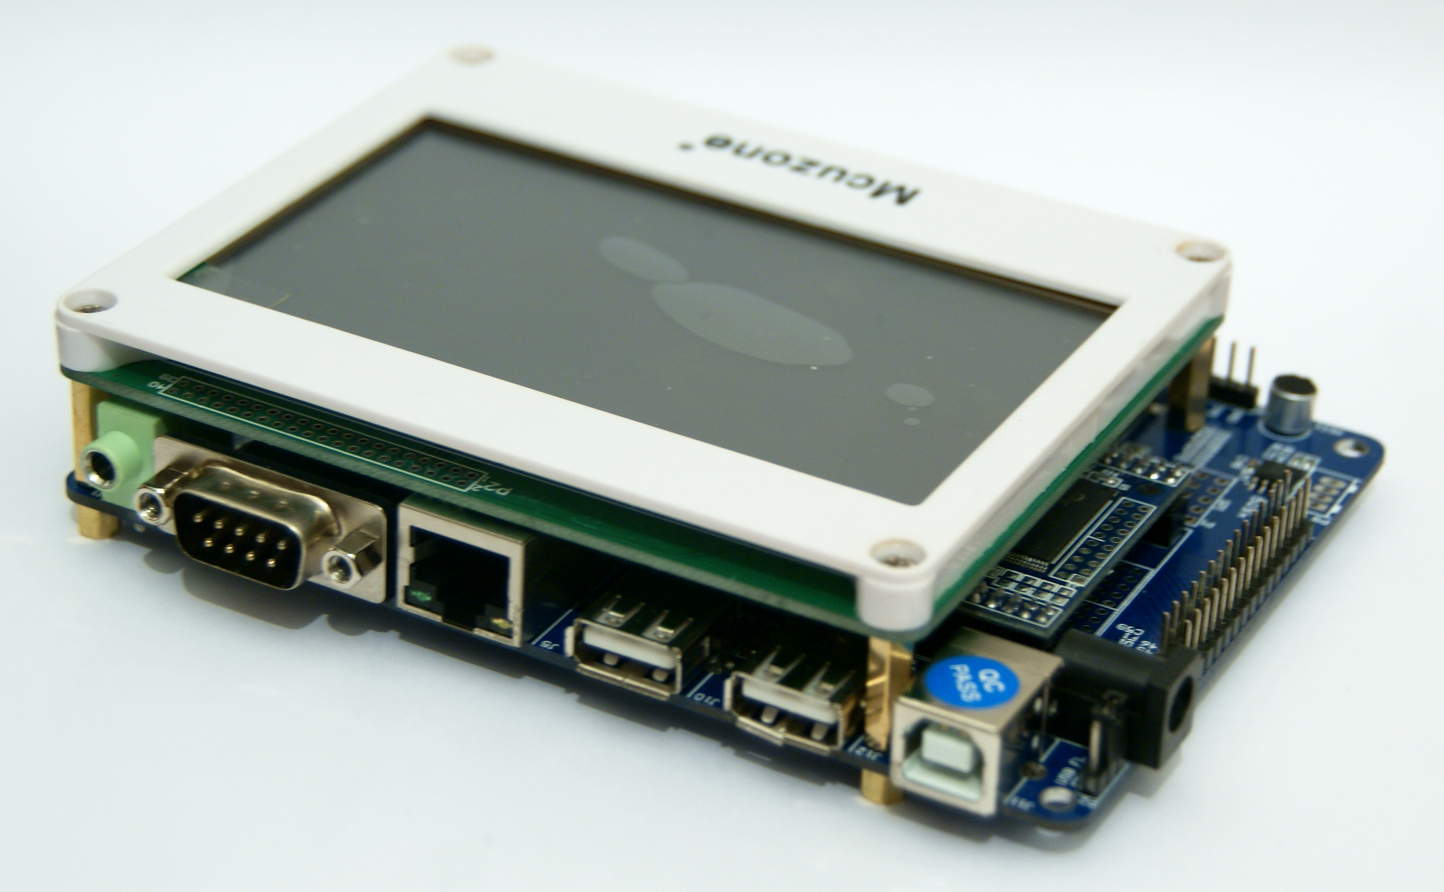
\includegraphics[height=0.4\textheight]{images/devkit.jpg}
  \end{center}
\end{frame}

\section{Concluding remarks}

\begin{frame}
  \begin{center}
    Thank you for your attention

    \vspace{0.15\textheight}

    {\Huge Questions?}

    \vspace{0.15\textheight}

    \href{mailto:luca@lucaceresoli.net}{luca@lucaceresoli.net}\\
    \url{http://lucaceresoli.net}

    \textcopyright{} Copyright 2017, Luca Ceresoli\\

    \vspace{0.05\textheight}

    \tiny
    Slides released under\\
    Creative Commons Attribution - Share Alike 3.0 License \\
    \url{https://creativecommons.org/licenses/by-sa/3.0/} \\
\end{center}
\end{frame}

\end{document}
